\documentclass{article}
\usepackage{tikz}
\usepackage[utf8]{inputenc}
\usepackage[all]{xy}

\title{Práctica 2: Autómatas finitos}
\author{Lothar Soto Palma DNI:49079173W}
\date{November 2014}

\begin{document}

\maketitle

\section*{Ejercicio 1}
Considere el siguiente AFD $M=(Q,A, \partial, q_{0}, F)$, donde:
\begin{itemize}

\item $Q=\{ q_{0}, q_{1},q_{2}\}$
\item $A=\{0,1\}$
\item La función de transición viene dada por:
$$\partial(q0, 0)= q1, \partial(q0, 1)= q0$$ $$\partial(q1, 0)= q2, \partial(q1, 1)= q0$$ $$\partial(q2, 0)= q2, \partial(q2, 1)= q2$$
\item $F=\{q_{2}\}$
Describa informalmente el lenguaje aceptado:
\end{itemize}
\begin{center}
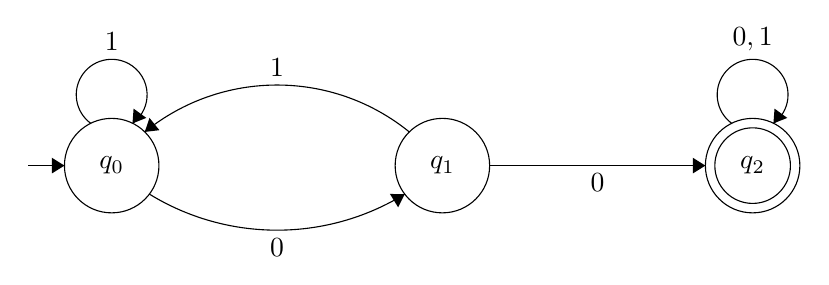
\begin{tikzpicture}[scale=0.2]
\tikzstyle{every node}+=[inner sep=0pt]
\draw [black] (14.4,-19.8) circle (3);
\draw (14.4,-19.8) node {$q_{0}$};
\draw [black] (35.4,-19.8) circle (3);
\draw (35.4,-19.8) node {$q_{1}$};
\draw [black] (55.1,-19.8) circle (3);
\draw (55.1,-19.8) node {$q_{2}$};
\draw [black] (55.1,-19.8) circle (2.4);
\draw [black] (38.4,-19.8) -- (52.1,-19.8);
\fill [black] (52.1,-19.8) -- (51.3,-19.3) -- (51.3,-20.3);
\draw (45.25,-20.3) node [below] {$0$};
\draw [black] (53.777,-17.12) arc (234:-54:2.25);
\draw (55.1,-12.55) node [above] {$0,1$};
\fill [black] (56.42,-17.12) -- (57.3,-16.77) -- (56.49,-16.18);
\draw [black] (33.011,-21.607) arc (-58.43339:-121.56661:15.495);
\fill [black] (33.01,-21.61) -- (32.07,-21.6) -- (32.59,-22.45);
\draw (24.9,-24.4) node [below] {$0$};
\draw [black] (16.497,-17.664) arc (129.07705:50.92295:13.33);
\fill [black] (16.5,-17.66) -- (17.43,-17.55) -- (16.8,-16.77);
\draw (24.9,-14.18) node [above] {$1$};
\draw [black] (13.077,-17.12) arc (234:-54:2.25);
\draw (14.4,-12.55) node [above] {$1$};
\fill [black] (15.72,-17.12) -- (16.6,-16.77) -- (15.79,-16.18);
\draw [black] (9.1,-19.8) -- (11.4,-19.8);
\fill [black] (11.4,-19.8) -- (10.6,-19.3) -- (10.6,-20.3);
\end{tikzpicture}
\end{center}

Solución:\\
$$L=1^*0(1^+0)^*0(1+0)^*$$\\
Son la palabras que tienen al menos dos 0. Puesto el diagrama permite la aparición de un 1 o no al comienzo de la cadena, entonces es necesario como mínimo dos 0 para llegar al estado $q_{2}$.

\section*{Ejercicio 2}
Dibujar los AFDs que aceptan los siguientes lenguajes con alfabeto $\{0,1\}$:
\begin{description}

\item[a)] El lenguaje vacío, $\emptyset$.
\begin{center}
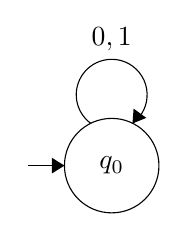
\begin{tikzpicture}[scale=0.2]
\tikzstyle{every node}+=[inner sep=0pt]
\draw [black] (29.3,-24) circle (3);
\draw (29.3,-24) node {$q_{0}$};
\draw [black] (24,-24) -- (26.3,-24);
\fill [black] (26.3,-24) -- (25.5,-23.5) -- (25.5,-24.5);
\draw [black] (27.977,-21.32) arc (234:-54:2.25);
\draw (29.3,-16.75) node [above] {$0,1$};
\fill [black] (30.62,-21.32) -- (31.5,-20.97) -- (30.69,-20.38);
\end{tikzpicture}
\end{center}

\item[b)] El lenguaje formado por la palabra , osea, vacía $\{\varepsilon\}$.
\begin{center}
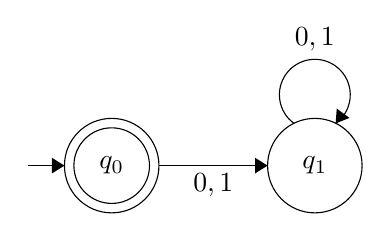
\begin{tikzpicture}[scale=0.2]
\tikzstyle{every node}+=[inner sep=0pt]
\draw [black] (29.3,-24) circle (3);
\draw (29.3,-24) node {$q_{0}$};
\draw [black] (29.3,-24) circle (2.4);
\draw [black] (42.2,-24) circle (3);
\draw (42.2,-24) node {$q_{1}$};
\draw [black] (24,-24) -- (26.3,-24);
\fill [black] (26.3,-24) -- (25.5,-23.5) -- (25.5,-24.5);
\draw [black] (32.3,-24) -- (39.2,-24);
\fill [black] (39.2,-24) -- (38.4,-23.5) -- (38.4,-24.5);
\draw (35.75,-24.5) node [below] {$0,1$};
\draw [black] (40.877,-21.32) arc (234:-54:2.25);
\draw (42.2,-16.75) node [above] {$0,1$};
\fill [black] (43.52,-21.32) -- (44.4,-20.97) -- (43.59,-20.38);
\end{tikzpicture}
\end{center}

\item[c)] El lenguaje formado por la palabra $01$, o sea, $\{01\}$.
\begin{center}
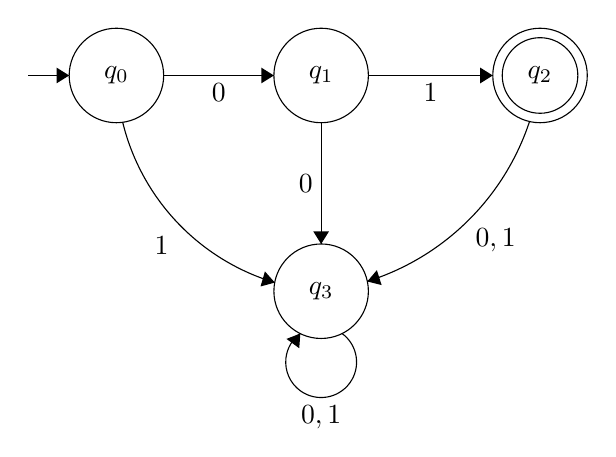
\begin{tikzpicture}[scale=0.2]
\tikzstyle{every node}+=[inner sep=0pt]
\draw [black] (19.9,-25.3) circle (3);
\draw (19.9,-25.3) node {$q_{0}$};
\draw [black] (32.9,-25.3) circle (3);
\draw (32.9,-25.3) node {$q_{1}$};
\draw [black] (46.8,-25.3) circle (3);
\draw (46.8,-25.3) node {$q_{2}$};
\draw [black] (46.8,-25.3) circle (2.4);
\draw [black] (32.9,-39) circle (3);
\draw (32.9,-39) node {$q_{3}$};
\draw [black] (22.9,-25.3) -- (29.9,-25.3);
\fill [black] (29.9,-25.3) -- (29.1,-24.8) -- (29.1,-25.8);
\draw (26.4,-25.8) node [below] {$0$};
\draw [black] (35.9,-25.3) -- (43.8,-25.3);
\fill [black] (43.8,-25.3) -- (43,-24.8) -- (43,-25.8);
\draw (39.85,-25.8) node [below] {$1$};
\draw [black] (29.957,-38.448) arc (-106.71344:-166.29014:14.124);
\fill [black] (29.96,-38.45) -- (29.33,-37.74) -- (29.05,-38.7);
\draw (23.24,-36.11) node [left] {$1$};
\draw [black] (32.9,-28.3) -- (32.9,-36);
\fill [black] (32.9,-36) -- (33.4,-35.2) -- (32.4,-35.2);
\draw (32.4,-32.15) node [left] {$0$};
\draw [black] (46.133,-28.22) arc (-18.28237:-72.54799:15.861);
\fill [black] (35.83,-38.38) -- (36.74,-38.61) -- (36.44,-37.66);
\draw (43.98,-35.02) node [below] {$0,1$};
\draw [black] (34.223,-41.68) arc (54:-234:2.25);
\draw (32.9,-46.25) node [below] {$0,1$};
\fill [black] (31.58,-41.68) -- (30.7,-42.03) -- (31.51,-42.62);
\draw [black] (14.3,-25.3) -- (16.9,-25.3);
\fill [black] (16.9,-25.3) -- (16.1,-24.8) -- (16.1,-25.8);
\end{tikzpicture}
\end{center}

\item[d)] El lenguaje $\{11,00\}$
\begin{center}
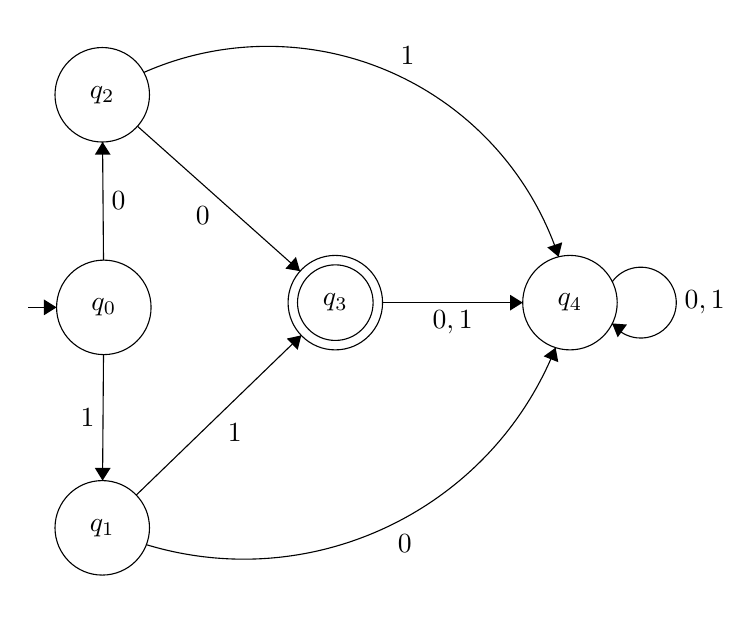
\begin{tikzpicture}[scale=0.2]
\tikzstyle{every node}+=[inner sep=0pt]
\draw [black] (24.1,-24.6) circle (3);
\draw (24.1,-24.6) node {$q_{0}$};
\draw [black] (24,-11.1) circle (3);
\draw (24,-11.1) node {$q_{2}$};
\draw [black] (24,-38.6) circle (3);
\draw (24,-38.6) node {$q_{1}$};
\draw [black] (38.8,-24.3) circle (3);
\draw (38.8,-24.3) node {$q_{3}$};
\draw [black] (38.8,-24.3) circle (2.4);
\draw [black] (53.7,-24.3) circle (3);
\draw (53.7,-24.3) node {$q_{4}$};
\draw [black] (24.08,-27.6) -- (24.02,-35.6);
\fill [black] (24.02,-35.6) -- (24.53,-34.8) -- (23.53,-34.8);
\draw (23.54,-31.6) node [left] {$1$};
\draw [black] (24.08,-21.6) -- (24.02,-14.1);
\fill [black] (24.02,-14.1) -- (23.53,-14.9) -- (24.53,-14.9);
\draw (24.56,-17.85) node [right] {$0$};
\draw [black] (26.24,-13.1) -- (36.56,-22.3);
\fill [black] (36.56,-22.3) -- (36.3,-21.4) -- (35.63,-22.14);
\draw (30.39,-18.19) node [below] {$0$};
\draw [black] (26.16,-36.52) -- (36.64,-26.38);
\fill [black] (36.64,-26.38) -- (35.72,-26.58) -- (36.41,-27.3);
\draw (32.42,-31.93) node [below] {$1$};
\draw [black] (41.8,-24.3) -- (50.7,-24.3);
\fill [black] (50.7,-24.3) -- (49.9,-23.8) -- (49.9,-24.8);
\draw (46.25,-24.8) node [below] {$0,1$};
\draw [black] (26.64,-9.682) arc (113.81804:18.25698:19.463);
\fill [black] (52.98,-21.39) -- (53.21,-20.47) -- (52.26,-20.79);
\draw (43.38,-9.19) node [above] {$1$};
\draw [black] (52.79,-27.156) arc (-21.71302:-106.86707:21.317);
\fill [black] (52.79,-27.16) -- (52.03,-27.71) -- (52.96,-28.08);
\draw (43.22,-38.98) node [below] {$0$};
\draw [black] (19.3,-24.6) -- (21.1,-24.6);
\fill [black] (21.1,-24.6) -- (20.3,-24.1) -- (20.3,-25.1);
\draw [black] (56.38,-22.977) arc (144:-144:2.25);
\draw (60.95,-24.3) node [right] {$0,1$};
\fill [black] (56.38,-25.62) -- (56.73,-26.5) -- (57.32,-25.69);
\end{tikzpicture}
\end{center}

\item[e)] El lenguaje formado por sucesiones de la subcadena ‘$01$’ incluyendo la cadena vacía, o sea, $\{\varepsilon, 01, 0101, 010101,...\}$
\begin{center}
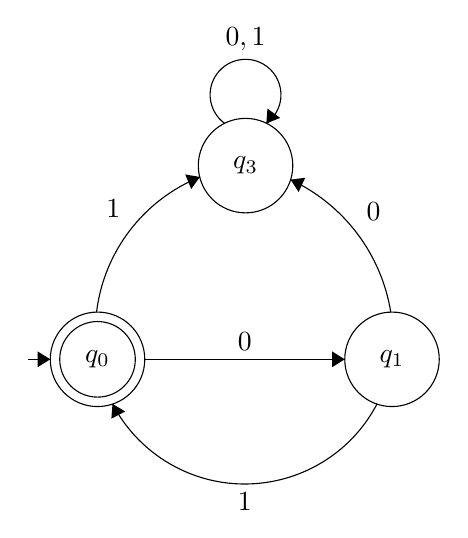
\begin{tikzpicture}[scale=0.2]
\tikzstyle{every node}+=[inner sep=0pt]
\draw [black] (16.9,-32) circle (3);
\draw (16.9,-32) node {$q_{0}$};
\draw [black] (16.9,-32) circle (2.4);
\draw [black] (35.6,-32) circle (3);
\draw (35.6,-32) node {$q_{1}$};
\draw [black] (26.3,-19.7) circle (3);
\draw (26.3,-19.7) node {$q_{3}$};
\draw [black] (19.9,-32) -- (32.6,-32);
\fill [black] (32.6,-32) -- (31.8,-31.5) -- (31.8,-32.5);
\draw (26.25,-31.5) node [above] {$0$};
\draw [black] (12.5,-32) -- (13.9,-32);
\fill [black] (13.9,-32) -- (13.1,-31.5) -- (13.1,-32.5);
\draw [black] (34.649,-34.832) arc (-27.62743:-152.37257:9.48);
\fill [black] (17.85,-34.83) -- (17.78,-35.77) -- (18.66,-35.31);
\draw (26.25,-40.42) node [below] {$1$};
\draw [black] (16.837,-29.011) arc (-186.87409:-247.90203:10.641);
\fill [black] (23.4,-20.42) -- (22.47,-20.26) -- (22.85,-21.19);
\draw (18.37,-22.42) node [left] {$1$};
\draw [black] (29.156,-20.59) arc (65.04821:9.13746:11.258);
\fill [black] (29.16,-20.59) -- (29.67,-21.38) -- (30.09,-20.47);
\draw (33.96,-22.61) node [right] {$0$};
\draw [black] (24.977,-17.02) arc (234:-54:2.25);
\draw (26.3,-12.45) node [above] {$0,1$};
\fill [black] (27.62,-17.02) -- (28.5,-16.67) -- (27.69,-16.08);
\end{tikzpicture}
\end{center}

\item[f)] El lenguaje formado por las cadenas donde el número de unos es divisible por $3$.
\begin{center}
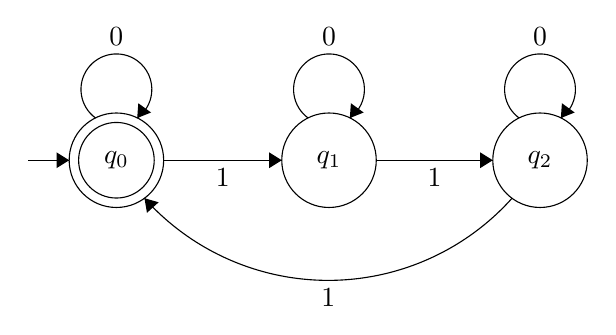
\begin{tikzpicture}[scale=0.2]
\tikzstyle{every node}+=[inner sep=0pt]
\draw [black] (19.9,-25.3) circle (3);
\draw (19.9,-25.3) node {$q_{0}$};
\draw [black] (19.9,-25.3) circle (2.4);
\draw [black] (33.4,-25.3) circle (3);
\draw (33.4,-25.3) node {$q_{1}$};
\draw [black] (46.8,-25.3) circle (3);
\draw (46.8,-25.3) node {$q_{2}$};
\draw [black] (22.9,-25.3) -- (30.4,-25.3);
\fill [black] (30.4,-25.3) -- (29.6,-24.8) -- (29.6,-25.8);
\draw (26.65,-25.8) node [below] {$1$};
\draw [black] (36.4,-25.3) -- (43.8,-25.3);
\fill [black] (43.8,-25.3) -- (43,-24.8) -- (43,-25.8);
\draw (40.1,-25.8) node [below] {$1$};
\draw [black] (14.3,-25.3) -- (16.9,-25.3);
\fill [black] (16.9,-25.3) -- (16.1,-24.8) -- (16.1,-25.8);
\draw [black] (32.077,-22.62) arc (234:-54:2.25);
\draw (33.4,-18.05) node [above] {$0$};
\fill [black] (34.72,-22.62) -- (35.6,-22.27) -- (34.79,-21.68);
\draw [black] (45.477,-22.62) arc (234:-54:2.25);
\draw (46.8,-18.05) node [above] {$0$};
\fill [black] (48.12,-22.62) -- (49,-22.27) -- (48.19,-21.68);
\draw [black] (18.577,-22.62) arc (234:-54:2.25);
\draw (19.9,-18.05) node [above] {$0$};
\fill [black] (21.22,-22.62) -- (22.1,-22.27) -- (21.29,-21.68);
\draw [black] (45.024,-27.712) arc (-41.84485:-138.15515:15.671);
\fill [black] (21.68,-27.71) -- (21.84,-28.64) -- (22.58,-27.97);
\draw (33.35,-33.43) node [below] {$1$};
\end{tikzpicture}
\end{center}
\end{description}

\section*{Ejercicio 3}
Dado el siguiente autómata M, describir el lenguaje aceptado por dicho autómata:
El lenguaje aceptado por este autómata es:
\begin{center}
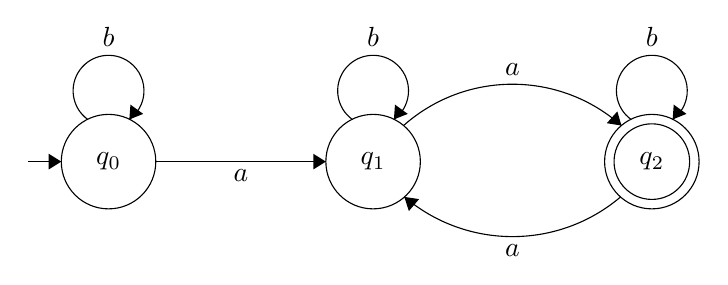
\begin{tikzpicture}[scale=0.2]
\tikzstyle{every node}+=[inner sep=0pt]
\draw [black] (24.2,-25.4) circle (3);
\draw (24.2,-25.4) node {$q_{0}$};
\draw [black] (41,-25.4) circle (3);
\draw (41,-25.4) node {$q_{1}$};
\draw [black] (58.7,-25.4) circle (3);
\draw (58.7,-25.4) node {$q_{2}$};
\draw [black] (58.7,-25.4) circle (2.4);
\draw [black] (42.927,-23.115) arc (131.61219:48.38781:10.424);
\fill [black] (56.77,-23.11) -- (56.51,-22.21) -- (55.84,-22.96);
\draw (49.85,-19.98) node [above] {$a$};
\draw [black] (56.718,-27.638) arc (-49.63596:-130.36404:10.604);
\fill [black] (42.98,-27.64) -- (43.27,-28.54) -- (43.92,-27.78);
\draw (49.85,-30.66) node [below] {$a$};
\draw [black] (27.2,-25.4) -- (38,-25.4);
\fill [black] (38,-25.4) -- (37.2,-24.9) -- (37.2,-25.9);
\draw (32.6,-25.9) node [below] {$a$};
\draw [black] (22.877,-22.72) arc (234:-54:2.25);
\draw (24.2,-18.15) node [above] {$b$};
\fill [black] (25.52,-22.72) -- (26.4,-22.37) -- (25.59,-21.78);
\draw [black] (39.677,-22.72) arc (234:-54:2.25);
\draw (41,-18.15) node [above] {$b$};
\fill [black] (42.32,-22.72) -- (43.2,-22.37) -- (42.39,-21.78);
\draw [black] (57.377,-22.72) arc (234:-54:2.25);
\draw (58.7,-18.15) node [above] {$b$};
\fill [black] (60.02,-22.72) -- (60.9,-22.37) -- (60.09,-21.78);
\draw [black] (19.1,-25.4) -- (21.2,-25.4);
\fill [black] (21.2,-25.4) -- (20.4,-24.9) -- (20.4,-25.9);
\end{tikzpicture}
\end{center}
Solcuión:\\
$$L=b^*ab^*ab^*(ab^*ab^*)^*$$\\
Son las cadenas con un número par de $a$. Inicia con $b^*$ puede comenzar con $b$ o directamente con $a$ pero es necesario al menos dos $a$ para llegar al estado final del autómata y formar una palabra.
\end{document}
